\documentclass[a4paper]{article}

\setlength{\parskip}{2mm}
\newcommand{\tab}{~ \qquad}
\usepackage{breqn}
\usepackage{ifthen}
\usepackage{amssymb}
\usepackage{multicol}
\usepackage{graphicx}
\usepackage[absolute]{textpos}
\usepackage{amsmath, amscd, amssymb, amsthm, latexsym}
% \usepackage[noload]{qtree}
%\usepackage{xspace,rotating,calligra,dsfont,ifthen}
\usepackage{xspace,rotating,dsfont,ifthen}
\usepackage[spanish,activeacute]{babel}
\usepackage[utf8]{inputenc}
\usepackage{pgfpages}
\usepackage{pgf,pgfarrows,pgfnodes,pgfautomata,pgfheaps,xspace,dsfont}
\usepackage{listings}
\usepackage{multicol}
\usepackage{todonotes}
\usepackage{url}
\usepackage{float}
\usepackage{framed,mdframed}
\usepackage{cancel}

\usepackage[strict]{changepage}


\makeatletter


\newcommand\hfrac[2]{\genfrac{}{}{0pt}{}{#1}{#2}} %\hfrac{}{} es un \frac sin la linea del medio

\newcommand\Wider[2][3em]{% \Wider[3em]{} reduce los m\'argenes
\makebox[\linewidth][c]{%
  \begin{minipage}{\dimexpr\textwidth+#1\relax}
  \raggedright#2
  \end{minipage}%
  }%
}


\@ifclassloaded{beamer}{%
  \newcommand{\tocarEspacios}{%
    \addtolength{\leftskip}{4em}%
    \addtolength{\parindent}{-3em}%
  }%
}
{%
  \usepackage[top=1cm,bottom=2cm,left=1cm,right=1cm]{geometry}%
  \usepackage{color}%
  \newcommand{\tocarEspacios}{%
    \addtolength{\leftskip}{3em}%
    \setlength{\parindent}{0em}%
  }%
}

\newcommand{\encabezadoDeProc}[4]{%
  % Ponemos la palabrita problema en tt
%  \noindent%
  {\normalfont\bfseries\ttfamily proc}%
  % Ponemos el nombre del problema
  \ %
  {\normalfont\ttfamily #2}%
  \
  % Ponemos los parametros
  (#3)%
  \ifthenelse{\equal{#4}{}}{}{%
  \ =\ %
  % Ponemos el nombre del resultado
  {\normalfont\ttfamily #1}%
  % Por ultimo, va el tipo del resultado
  \ : #4}
}

\newcommand{\encabezadoDeTipo}[2]{%
  % Ponemos la palabrita tipo en tt
  {\normalfont\bfseries\ttfamily tipo}%
  % Ponemos el nombre del tipo
  \ %
  {\normalfont\ttfamily #2}%
  \ifthenelse{\equal{#1}{}}{}{$\langle$#1$\rangle$}
}

% Primero definiciones de cosas al estilo title, author, date

\def\materia#1{\gdef\@materia{#1}}
\def\@materia{No especifi\'o la materia}
\def\lamateria{\@materia}

\def\cuatrimestre#1{\gdef\@cuatrimestre{#1}}
\def\@cuatrimestre{No especifi\'o el cuatrimestre}
\def\elcuatrimestre{\@cuatrimestre}

\def\anio#1{\gdef\@anio{#1}}
\def\@anio{No especifi\'o el anio}
\def\elanio{\@anio}

\def\fecha#1{\gdef\@fecha{#1}}
\def\@fecha{\today}
\def\lafecha{\@fecha}

\def\nombre#1{\gdef\@nombre{#1}}
\def\@nombre{No especific'o el nombre}
\def\elnombre{\@nombre}

\def\practicas#1{\gdef\@practica{#1}}
\def\@practica{No especifi\'o el n\'umero de pr\'actica}
\def\lapractica{\@practica}


% Esta macro convierte el numero de cuatrimestre a palabras
\newcommand{\cuatrimestreLindo}{
  \ifthenelse{\equal{\elcuatrimestre}{1}}
  {Primer cuatrimestre}
  {\ifthenelse{\equal{\elcuatrimestre}{2}}
  {Segundo cuatrimestre}
  {Verano}}
}


\newcommand{\depto}{{UBA -- Facultad de Ciencias Exactas y Naturales --
      Departamento de Computaci\'on}}

\newcommand{\titulopractica}{
  \centerline{\depto}
  \vspace{1ex}
  \centerline{{\Large\lamateria}}
  \vspace{0.5ex}
  \centerline{\cuatrimestreLindo de \elanio}
  \vspace{2ex}
  \centerline{{\huge Pr\'actica \lapractica -- \elnombre}}
  \vspace{5ex}
  \arreglarincisos
  \newcounter{ejercicio}
  \newenvironment{ejercicio}{\stepcounter{ejercicio}\textbf{Ejercicio
      \theejercicio}%
    \renewcommand\@currentlabel{\theejercicio}%
  }{\vspace{0.2cm}}
}


\newcommand{\titulotp}{
  \centerline{\depto}
  \vspace{1ex}
  \centerline{{\Large\lamateria}}
  \vspace{0.5ex}
  \centerline{\cuatrimestreLindo de \elanio}
  \vspace{0.5ex}
  \centerline{\lafecha}
  \vspace{2ex}
  \centerline{{\huge\elnombre}}
  \vspace{5ex}
}


%practicas
\newcommand{\practica}[2]{%
    \title{Pr\'actica #1 \\ #2}
    \author{Algoritmos y Estructuras de Datos I}
    \date{Primer Cuatrimestre 2022}

    \maketitlepractica{#1}{#2}
}

\newcommand \maketitlepractica[2] {%
\begin{center}
\begin{tabular}{r cr}
 \begin{tabular}{c}
{\large\bf\textsf{\ Algoritmos y Estructuras de Datos I\ }}\\
Primer Cuatrimestre 2022\\
\title{\normalsize Gu\'ia Pr\'actica #1 \\ \textbf{#2}}\\
\@title
\end{tabular} &
\begin{tabular}{@{} p{1.6cm} @{}}
\includegraphics[width=1.6cm]{logodpt.jpg}
\end{tabular} &
\begin{tabular}{l @{}}
 \emph{Departamento de Computaci\'on} \\
 \emph{Facultad de Ciencias Exactas y Naturales} \\
 \emph{Universidad de Buenos Aires} \\
\end{tabular}
\end{tabular}
\end{center}

\bigskip
}


% Símbolos varios

\newcommand{\nat}{\ensuremath{\mathds{N}}}
\newcommand{\ent}{\ensuremath{\mathds{Z}}}
\newcommand{\float}{\ensuremath{\mathds{R}}}
\newcommand{\bool}{\ensuremath{\mathsf{Bool}}}
\newcommand{\True}{\ensuremath{\mathrm{true}}}
\newcommand{\False}{\ensuremath{\mathrm{false}}}
\newcommand{\Then}{\ensuremath{\rightarrow}}
\newcommand{\Iff}{\ensuremath{\leftrightarrow}}
\newcommand{\implica}{\ensuremath{\longrightarrow}}
\newcommand{\IfThenElse}[3]{\ensuremath{\mathsf{if}\ #1\ \mathsf{then}\ #2\ \mathsf{else}\ #3\ \mathsf{fi}}}
\newcommand{\In}{\textsf{in }}
\newcommand{\Out}{\textsf{out }}
\newcommand{\Inout}{\textsf{inout }}
\newcommand{\yLuego}{\hspace{6pt} \land _L \hspace{6pt}}
\newcommand{\oLuego}{\hspace{6pt} \lor _L \hspace{6pt}}
\newcommand{\implicaLuego}{\implica _L }
\newcommand{\cuantificador}[5]{%
	\ensuremath{(#2 #3: #4)\ (%
		\ifthenelse{\equal{#1}{unalinea}}{
			#5
		}{
			$ % exiting math mode
			\begin{adjustwidth}{+2em}{}
			$#5$%
			\end{adjustwidth}%
			$ % entering math mode
		}
	)}
}

\newcommand{\existe}[4][]{%
	\cuantificador{#1}{\exists}{#2}{#3}{#4}
}
\newcommand{\paraTodo}[4][]{%
	\cuantificador{#1}{\forall}{#2}{#3}{#4}
}

% Símbolo para marcar los ejercicios importantes (estrellita)
\newcommand\importante{\raisebox{0.5pt}{\ensuremath{\bigstar}}}


\newcommand{\rango}[2]{[#1\twodots#2]}
\newcommand{\comp}[2]{[\,#1\,|\,#2\,]}

\newcommand{\rangoac}[2]{(#1\twodots#2]}
\newcommand{\rangoca}[2]{[#1\twodots#2)}
\newcommand{\rangoaa}[2]{(#1\twodots#2)}

%ejercicios
\newtheorem{exercise}{Ejercicio}
\newenvironment{ejercicio}[1][]{\begin{exercise}#1\rm}{\end{exercise} \vspace{0.2cm}}
\newenvironment{items}{\begin{enumerate}[a)]}{\end{enumerate}}
\newenvironment{subitems}{\begin{enumerate}[i)]}{\end{enumerate}}
\newcommand{\sugerencia}[1]{\noindent \textbf{Sugerencia:} #1}

\lstnewenvironment{code}{
    \lstset{% general command to set parameter(s)
        language=C++, basicstyle=\small\ttfamily, keywordstyle=\slshape,
        emph=[1]{tipo,usa}, emphstyle={[1]\sffamily\bfseries},
        morekeywords={tint,forn,forsn},
        basewidth={0.47em,0.40em},
        columns=fixed, fontadjust, resetmargins, xrightmargin=5pt, xleftmargin=15pt,
        flexiblecolumns=false, tabsize=2, breaklines, breakatwhitespace=false, extendedchars=true,
        numbers=left, numberstyle=\tiny, stepnumber=1, numbersep=9pt,
        frame=l, framesep=3pt,
    }
   \csname lst@SetFirstLabel\endcsname}
  {\csname lst@SaveFirstLabel\endcsname}


%tipos basicos
\newcommand{\rea}{\ensuremath{\mathsf{Float}}}
\newcommand{\cha}{\ensuremath{\mathsf{Char}}}
\newcommand{\str}{\ensuremath{\mathsf{String}}}

\newcommand{\mcd}{\mathrm{mcd}}
\newcommand{\prm}[1]{\ensuremath{\mathsf{prm}(#1)}}
\newcommand{\sgd}[1]{\ensuremath{\mathsf{sgd}(#1)}}

\newcommand{\tuple}[2]{\ensuremath{#1 \times #2}}

%listas
\newcommand{\TLista}[1]{\ensuremath{seq \langle #1\rangle}}
\newcommand{\lvacia}{\ensuremath{[\ ]}}
\newcommand{\lv}{\ensuremath{[\ ]}}
\newcommand{\longitud}[1]{\ensuremath{|#1|}}
\newcommand{\cons}[1]{\ensuremath{\mathsf{addFirst}}(#1)}
\newcommand{\indice}[1]{\ensuremath{\mathsf{indice}}(#1)}
\newcommand{\conc}[1]{\ensuremath{\mathsf{concat}}(#1)}
\newcommand{\cab}[1]{\ensuremath{\mathsf{head}}(#1)}
\newcommand{\cola}[1]{\ensuremath{\mathsf{tail}}(#1)}
\newcommand{\sub}[1]{\ensuremath{\mathsf{subseq}}(#1)}
\newcommand{\en}[1]{\ensuremath{\mathsf{en}}(#1)}
\newcommand{\cuenta}[2]{\mathsf{cuenta}\ensuremath{(#1, #2)}}
\newcommand{\suma}[1]{\mathsf{suma}(#1)}
\newcommand{\twodots}{\ensuremath{\mathrm{..}}}
\newcommand{\masmas}{\ensuremath{++}}
\newcommand{\matriz}[1]{\TLista{\TLista{#1}}}

\newcommand{\seqchar}{\TLista{\cha}}


% Acumulador
\newcommand{\acum}[1]{\ensuremath{\mathsf{acum}}(#1)}
\newcommand{\acumselec}[3]{\ensuremath{\mathrm{acum}(#1 |  #2, #3)}}

% \selector{variable}{dominio}
\newcommand{\selector}[2]{#1~\ensuremath{\leftarrow}~#2}
\newcommand{\selec}{\ensuremath{\leftarrow}}

\newcommand{\pred}[3]{%
    {\normalfont\bfseries\ttfamily\noindent pred }%
    {\normalfont\ttfamily #1}%
    \ifthenelse{\equal{#2}{}}{}{\ (#2) }%
    \{%
    \begin{adjustwidth}{+2em}{}
      \ensuremath{#3}
    \end{adjustwidth}
    \}%
    {\normalfont\bfseries\,\par}%
}

\newenvironment{proc}[4][res]{%

  % El parametro 1 (opcional) es el nombre del resultado
  % El parametro 2 es el nombre del problema
  % El parametro 3 son los parametros
  % El parametro 4 es el tipo del resultado
  % Preambulo del ambiente problema
  % Tenemos que definir los comandos requiere, asegura, modifica y aux
  \newcommand{\pre}[2][]{%
    {\normalfont\bfseries\ttfamily Pre}%
    \ifthenelse{\equal{##1}{}}{}{\ {\normalfont\ttfamily ##1} :}\ %
    \{\ensuremath{##2}\}%
    {\normalfont\bfseries\,\par}%
  }
  \newcommand{\post}[2][]{%
    {\normalfont\bfseries\ttfamily Post}%
    \ifthenelse{\equal{##1}{}}{}{\ {\normalfont\ttfamily ##1} :}\
    \{\ensuremath{##2}\}%
    {\normalfont\bfseries\,\par}%
  }
  \renewcommand{\aux}[4]{%
    {\normalfont\bfseries\ttfamily aux\ }%
    {\normalfont\ttfamily ##1}%
    \ifthenelse{\equal{##2}{}}{}{\ (##2)}\ : ##3\, = \ensuremath{##4}%
    {\normalfont\bfseries\,;\par}%
  }
  \renewcommand{\pred}[3]{%
    {\normalfont\bfseries\ttfamily pred }%
    {\normalfont\ttfamily ##1}%
    \ifthenelse{\equal{##2}{}}{}{\ (##2) }%
    \{%
    \begin{adjustwidth}{+5em}{}
      \ensuremath{##3}
    \end{adjustwidth}
    \}%
    {\normalfont\bfseries\,\par}%
  }

  \newcommand{\res}{#1}
  \vspace{1ex}
  \noindent
  \encabezadoDeProc{#1}{#2}{#3}{#4}
  % Abrimos la llave
  \{\par%
  \tocarEspacios
}
% Ahora viene el cierre del ambiente problema
{
  % Cerramos la llave
  \noindent\}
  \vspace{1ex}
}


\newcommand{\aux}[4]{%
    {\normalfont\bfseries\ttfamily\noindent aux\ }%
    {\normalfont\ttfamily #1}%
    \ifthenelse{\equal{#2}{}}{}{\ (#2)}\ : #3\, = \ensuremath{#4}%
    {\normalfont\bfseries\,;\par}%
}


% \newcommand{\pre}[1]{\textsf{pre}\ensuremath{(#1)}}

\newcommand{\procnom}[1]{\textsf{#1}}
\newcommand{\procil}[3]{\textsf{proc #1}\ensuremath{(#2) = #3}}
\newcommand{\procilsinres}[2]{\textsf{proc #1}\ensuremath{(#2)}}
\newcommand{\preil}[2]{\textsf{Pre #1: }\ensuremath{#2}}
\newcommand{\postil}[2]{\textsf{Post #1: }\ensuremath{#2}}
\newcommand{\auxil}[2]{\textsf{fun }\ensuremath{#1 = #2}}
\newcommand{\auxilc}[4]{\textsf{fun }\ensuremath{#1( #2 ): #3 = #4}}
\newcommand{\auxnom}[1]{\textsf{fun }\ensuremath{#1}}
\newcommand{\auxpred}[3]{\textsf{pred }\ensuremath{#1( #2 ) \{ #3 \}}}

\newcommand{\comentario}[1]{\text{/*\ #1\ */}}

\newcommand{\nom}[1]{\ensuremath{\mathsf{#1}}}


% En las practicas/parciales usamos numeros arabigos para los ejercicios.
% Aca cambiamos los enumerate comunes para que usen letras y numeros
% romanos
\newcommand{\arreglarincisos}{%
  \renewcommand{\theenumi}{\alph{enumi}}
  \renewcommand{\theenumii}{\roman{enumii}}
  \renewcommand{\labelenumi}{\theenumi)}
  \renewcommand{\labelenumii}{\theenumii)}
}



%%%%%%%%%%%%%%%%%%%%%%%%%%%%%% PARCIAL %%%%%%%%%%%%%%%%%%%%%%%%
\let\@xa\expandafter
\newcommand{\tituloparcial}{\centerline{\depto -- \lamateria}
  \centerline{\elnombre -- \lafecha}%
  \setlength{\TPHorizModule}{10mm} % Fija las unidades de textpos
  \setlength{\TPVertModule}{\TPHorizModule} % Fija las unidades de
                                % textpos
  \arreglarincisos
  \newcounter{total}% Este contador va a guardar cuantos incisos hay
                    % en el parcial. Si un ejercicio no tiene incisos,
                    % cuenta como un inciso.
  \newcounter{contgrilla} % Para hacer ciclos
  \newcounter{columnainicial} % Se van a usar para los cline cuando un
  \newcounter{columnafinal}   % ejercicio tenga incisos.
  \newcommand{\primerafila}{}
  \newcommand{\segundafila}{}
  \newcommand{\rayitas}{} % Esto va a guardar los \cline de los
                          % ejercicios con incisos, asi queda mas bonito
  \newcommand{\anchodegrilla}{20} % Es para textpos
  \newcommand{\izquierda}{7} % Estos dos le dicen a textpos donde colocar
  \newcommand{\abajo}{2}     % la grilla
  \newcommand{\anchodecasilla}{0.4cm}
  \setcounter{columnainicial}{1}
  \setcounter{total}{0}
  \newcounter{ejercicio}
  \setcounter{ejercicio}{0}
  \renewenvironment{ejercicio}[1]
  {%
    \stepcounter{ejercicio}\textbf{\noindent Ejercicio \theejercicio. [##1
      puntos]}% Formato
    \renewcommand\@currentlabel{\theejercicio}% Esto es para las
                                % referencias
    \newcommand{\invariante}[2]{%
      {\normalfont\bfseries\ttfamily invariante}%
      \ ####1\hspace{1em}####2%
    }%
    \newcommand{\Proc}[5][result]{
      \encabezadoDeProc{####1}{####2}{####3}{####4}\hspace{1em}####5}%
  }% Aca se termina el principio del ejercicio
  {% Ahora viene el final
    % Esto suma la cantidad de incisos o 1 si no hubo ninguno
    \ifthenelse{\equal{\value{enumi}}{0}}
    {\addtocounter{total}{1}}
    {\addtocounter{total}{\value{enumi}}}
    \ifthenelse{\equal{\value{ejercicio}}{1}}{}
    {
      \g@addto@macro\primerafila{&} % Si no estoy en el primer ej.
      \g@addto@macro\segundafila{&}
    }
    \ifthenelse{\equal{\value{enumi}}{0}}
    {% No tiene incisos
      \g@addto@macro\primerafila{\multicolumn{1}{|c|}}
      \bgroup% avoid overwriting somebody else's value of \tmp@a
      \protected@edef\tmp@a{\theejercicio}% expand as far as we can
      \@xa\g@addto@macro\@xa\primerafila\@xa{\tmp@a}%
      \egroup% restore old value of \tmp@a, effect of \g@addto.. is

      \stepcounter{columnainicial}
    }
    {% Tiene incisos
      % Primero ponemos el encabezado
      \g@addto@macro\primerafila{\multicolumn}% Ahora el numero de items
      \bgroup% avoid overwriting somebody else's value of \tmp@a
      \protected@edef\tmp@a{\arabic{enumi}}% expand as far as we can
      \@xa\g@addto@macro\@xa\primerafila\@xa{\tmp@a}%
      \egroup% restore old value of \tmp@a, effect of \g@addto.. is
      % global
      % Ahora el formato
      \g@addto@macro\primerafila{{|c|}}%
      % Ahora el numero de ejercicio
      \bgroup% avoid overwriting somebody else's value of \tmp@a
      \protected@edef\tmp@a{\theejercicio}% expand as far as we can
      \@xa\g@addto@macro\@xa\primerafila\@xa{\tmp@a}%
      \egroup% restore old value of \tmp@a, effect of \g@addto.. is
      % global
      % Ahora armamos la segunda fila
      \g@addto@macro\segundafila{\multicolumn{1}{|c|}{a}}%
      \setcounter{contgrilla}{1}
      \whiledo{\value{contgrilla}<\value{enumi}}
      {%
        \stepcounter{contgrilla}
        \g@addto@macro\segundafila{&\multicolumn{1}{|c|}}
        \bgroup% avoid overwriting somebody else's value of \tmp@a
        \protected@edef\tmp@a{\alph{contgrilla}}% expand as far as we can
        \@xa\g@addto@macro\@xa\segundafila\@xa{\tmp@a}%
        \egroup% restore old value of \tmp@a, effect of \g@addto.. is
        % global
      }
      % Ahora armo las rayitas
      \setcounter{columnafinal}{\value{columnainicial}}
      \addtocounter{columnafinal}{-1}
      \addtocounter{columnafinal}{\value{enumi}}
      \bgroup% avoid overwriting somebody else's value of \tmp@a
      \protected@edef\tmp@a{\noexpand\cline{%
          \thecolumnainicial-\thecolumnafinal}}%
      \@xa\g@addto@macro\@xa\rayitas\@xa{\tmp@a}%
      \egroup% restore old value of \tmp@a, effect of \g@addto.. is
      \setcounter{columnainicial}{\value{columnafinal}}
      \stepcounter{columnainicial}
    }
    \setcounter{enumi}{0}%
    \vspace{0.2cm}%
  }%
  \newcommand{\tercerafila}{}
  \newcommand{\armartercerafila}{
    \setcounter{contgrilla}{1}
    \whiledo{\value{contgrilla}<\value{total}}
    {\stepcounter{contgrilla}\g@addto@macro\tercerafila{&}}
  }
  \newcommand{\grilla}{%
    \g@addto@macro\primerafila{&\textbf{TOTAL}}
    \g@addto@macro\segundafila{&}
    \g@addto@macro\tercerafila{&}
    \armartercerafila
    \ifthenelse{\equal{\value{total}}{\value{ejercicio}}}
    {% No hubo incisos
      \begin{textblock}{\anchodegrilla}(\izquierda,\abajo)
        \begin{tabular}{|*{\value{total}}{p{\anchodecasilla}|}c|}
          \hline
          \primerafila\\
          \hline
          \tercerafila\\
          \tercerafila\\
          \hline
        \end{tabular}
      \end{textblock}
    }
    {% Hubo incisos
      \begin{textblock}{\anchodegrilla}(\izquierda,\abajo)
        \begin{tabular}{|*{\value{total}}{p{\anchodecasilla}|}c|}
          \hline
          \primerafila\\
          \rayitas
          \segundafila\\
          \hline
          \tercerafila\\
          \tercerafila\\
          \hline
        \end{tabular}
      \end{textblock}
    }
  }%
  % \datosalumno
}

\newcommand{\datosalumno}{
  \vspace{0.4cm}
  \textbf{Apellidos:}

  \textbf{Nombres:}

  \textbf{LU:}

  \textbf{Correo electrónico:}

  \textbf{Nro. de carillas que adjunta:}
  \vspace{0.5cm}
}


% AMBIENTE CONSIGNAS
% Se usa en el TP para ir agregando las cosas que tienen que resolver
% los alumnos.
% Dentro del ambiente hay que usar \item para cada consigna

\newcounter{consigna}
\setcounter{consigna}{0}

\newenvironment{consignas}{%
  \newcommand{\consigna}{\stepcounter{consigna}\textbf{\theconsigna.}}%
  \renewcommand{\ejercicio}[1]{\item ##1 }
  \renewcommand{\proc}[5][result]{\item
    \encabezadoDeProc{##1}{##2}{##3}{##4}\hspace{1em}##5}%
  \newcommand{\invariante}[2]{\item%
    {\normalfont\bfseries\ttfamily invariante}%
    \ ##1\hspace{1em}##2%
  }
  \renewcommand{\aux}[4]{\item%
    {\normalfont\bfseries\ttfamily aux\ }%
    {\normalfont\ttfamily ##1}%
    \ifthenelse{\equal{##2}{}}{}{\ (##2)}\ : ##3 \hspace{1em}##4%
  }
  % Comienza la lista de consignas
  \begin{list}{\consigna}{%
      \setlength{\itemsep}{0.5em}%
      \setlength{\parsep}{0cm}%
    }
}%
{\end{list}}



% para decidir si usar && o ^
\newcommand{\y}[0]{\hspace{4pt} \ensuremath{\land} \hspace{4pt}}
\newcommand{\oo}[0]{\hspace{4pt} \ensuremath{\lor} \hspace{4pt}}

% macros de correctitud
\newcommand{\semanticComment}[2]{#1 \ensuremath{#2};}
\newcommand{\namedSemanticComment}[3]{#1 #2: \ensuremath{#3};}


\newcommand{\local}[1]{\semanticComment{local}{#1}}

\newcommand{\vale}[1]{\semanticComment{vale}{#1}}
\newcommand{\valeN}[2]{\namedSemanticComment{vale}{#1}{#2}}
\newcommand{\impl}[1]{\semanticComment{implica}{#1}}
\newcommand{\implN}[2]{\namedSemanticComment{implica}{#1}{#2}}
\newcommand{\estado}[1]{\semanticComment{estado}{#1}}

\newcommand{\invarianteCN}[2]{\namedSemanticComment{invariante}{#1}{#2}}
\newcommand{\invarianteC}[1]{\semanticComment{invariante}{#1}}
\newcommand{\varianteCN}[2]{\namedSemanticComment{variante}{#1}{#2}}
\newcommand{\varianteC}[1]{\semanticComment{variante}{#1}}

\usepackage{caratula} % Version modificada para usar las macros de algo1 de ~> https://github.com/bcardiff/dc-tex
\usepackage{graphicx}
\usepackage{booktabs}
\usepackage{amsmath}
\usepackage{amssymb}

\begin{document}

\titulo{Optimización de Rendimiento en Arquitecturas de Computadoras}
\subtitulo{Análisis Comparativo de Técnicas de Aceleración}
\fecha{30 de Agosto de 2025}
\materia{Organización del Computador II}
\grupo{Grupo 1}

\integrante{Polonuer, Joaquin}{1612/21}{jtpolonuer@gmail.com}

\maketitle

\tableofcontents
\newpage

\section{Introducción}

\subsection{La Ecuación de Onda}

La ecuación de onda representa uno de los fenómenos físicos más fundamentales en la naturaleza, describiendo la propagación de perturbaciones en medios continuos. Desde ondas sonoras y electromagnéticas hasta vibraciones mecánicas, este modelo matemático encuentra aplicación en campos tan diversos como la acústica, la óptica, la sismología y la ingeniería estructural.

\subsubsection{Ecuación de Onda en Una Dimensión}

La ecuación de onda unidimensional se expresa como:

\begin{equation}
    \frac{\partial^2 u}{\partial t^2} = c^2 \frac{\partial^2 u}{\partial x^2}
\end{equation}

donde $u(x,t)$ representa el desplazamiento de la onda en el punto $x$ y tiempo $t$, y $c$ es la velocidad de propagación característica del medio. Esta ecuación diferencial parcial de segundo orden describe fenómenos como:

\begin{itemize}
    \item Vibraciones de cuerdas tensadas
    \item Propagación de ondas sonoras en tubos
    \item Ondas electromagnéticas en líneas de transmisión
\end{itemize}

\subsubsection{Ecuación de Onda en Dos Dimensiones}

La extensión a dos dimensiones espaciales resulta en:

\begin{equation}
    \frac{\partial^2 u}{\partial t^2} = c^2 \left(\frac{\partial^2 u}{\partial x^2} + \frac{\partial^2 u}{\partial y^2}\right) = c^2 \nabla^2 u
\end{equation}

Esta formulación bidimensional modela fenómenos como:

\begin{itemize}
    \item Vibraciones de membranas (tambores, diafragmas)
    \item Ondas superficiales en líquidos
    \item Propagación de ondas sísmicas en planos
    \item Ondas electromagnéticas en cavidades rectangulares
\end{itemize}

La solución numérica de estas ecuaciones mediante métodos de diferencias finitas o elementos finitos requiere algoritmos computacionalmente intensivos que se benefician significativamente de técnicas de optimización.

\subsection{La Transformada de Fourier}

La Transformada de Fourier constituye una herramienta matemática fundamental para el análisis de fenómenos ondulatorios, permitiendo
descomponer señales complejas en sus componentes frecuenciales básicas. Esta transformación resulta especialmente poderosa en el
contexto de la resolución de ecuaciones diferenciales parciales.

La Transformada de Fourier continua de una función $f(x)$ se define como:

\begin{equation}
    F(\omega) = \int_{-\infty}^{\infty} f(x) e^{-j\omega x} dx
\end{equation}

y su transformada inversa:

\begin{equation}
    f(x) = \frac{1}{2\pi} \int_{-\infty}^{\infty} F(\omega) e^{j\omega x} d\omega
\end{equation}

Esta representación en el dominio frecuencial revela propiedades fundamentales de las señales y simplifica considerablemente el
análisis de sistemas lineales.

\subsection{Resolución de la Ecuación de Onda mediante la Transformada de Fourier}

La aplicación de la Transformada de Fourier a la ecuación de onda trasforma el problema diferencial en uno algebraico, facilitando
significativamente su resolución. Considerando la ecuación de onda unidimensional con condiciones iniciales:

\begin{equation}
    \frac{\partial^2 u}{\partial t^2} = c^2 \frac{\partial^2 u}{\partial x^2}
\end{equation}

Al aplicar la Transformada de Fourier espacial, obtenemos:

\begin{equation}
    \frac{\partial^2 \hat{u}}{\partial t^2} = -c^2 \omega^2 \hat{u}
\end{equation}

donde $\hat{u}(\omega, t)$ es la transformada de Fourier de $u(x,t)$ respecto a $x$. Esta ecuación diferencial ordinaria en el
tiempo tiene solución analítica conocida:

\begin{equation}
    \hat{u}(\omega, t) = A(\omega) e^{jc\omega t} + B(\omega) e^{-jc\omega t}
\end{equation}

Los coeficientes $A(\omega)$ y $B(\omega)$ se determinan a partir de las condiciones iniciales, y la solución final se obtiene
aplicando la transformada inversa de Fourier.

Esta metodología demuestra la potencia computacional de la Transformada de Fourier, convirtiendo operaciones de derivación en
multiplicaciones algebraicas simples. En implementaciones numéricas, la eficiencia de algoritmos FFT (Fast Fourier Transform)
resulta crítica para la viabilidad computacional de estos métodos espectrales.

El marco teórico se fundamenta en los principios de arquitectura de computadoras y optimización de código aplicados específicamente
a algoritmos de procesamiento de señales. Las aplicaciones similares en el campo científico e industrial incluyen bibliotecas de
álgebra lineal optimizadas como BLAS \cite{lawson1979basic}, implementaciones optimizadas de FFT como FFTW \cite{frigo2005design},
frameworks de computación paralela como OpenMP \cite{dagum1998openmp}, y compiladores optimizantes que emplean técnicas avanzadas de
análisis estático \cite{muchnick1997advanced}.

\subsection{Transformada Discreta de Fourier}

Para implementaciones computacionales, la Transformada de Fourier continua debe discretizarse. La Transformada Discreta de Fourier
(DFT) de una secuencia finita $x[n]$ de $N$ elementos se define como:

\begin{equation}
    X[k] = \sum_{n=0}^{N-1} x[n] e^{-j2\pi kn/N}, \quad k = 0, 1, \ldots, N-1
\end{equation}

donde $X[k]$ representa los coeficientes espectrales discretos. La transformada inversa se expresa como:

\begin{equation}
    x[n] = \frac{1}{N} \sum_{k=0}^{N-1} X[k] e^{j2\pi kn/N}, \quad n = 0, 1, \ldots, N-1
\end{equation}

La implementación directa de la DFT requiere $O(N^2)$ operaciones complejas, lo que resulta computacionalmente prohibitivo para
secuencias largas. Esta limitación motivó el desarrollo del algoritmo Fast Fourier Transform.

\subsection{Transformada Rápida de Fourier (Cooley-Tukey)}

El algoritmo FFT, desarrollado por Cooley y Tukey en 1965, reduce la complejidad computacional de $O(N^2)$ a $O(N \log N)$ mediante
la estrategia de divide y vencerás. Para $N = 2^m$, el algoritmo descompone la DFT en DFTs más pequeñas.

El algoritmo DIT (Decimation-in-Time) separa la secuencia de entrada en muestras pares e impares:

\begin{equation}
    X[k] = \sum_{n \text{ par}} x[n] e^{-j2\pi kn/N} + \sum_{n \text{ impar}} x[n] e^{-j2\pi kn/N}
\end{equation}

Sustituyendo $n = 2r$ para índices pares y $n = 2r+1$ para impares:

\begin{equation}
    X[k] = \sum_{r=0}^{N/2-1} x[2r] e^{-j2\pi kr/(N/2)} + e^{-j2\pi k/N} \sum_{r=0}^{N/2-1} x[2r+1] e^{-j2\pi kr/(N/2)}
\end{equation}

Definiendo:
\begin{align}
    X_{\text{par}}[k]   & = \sum_{r=0}^{N/2-1} x[2r] e^{-j2\pi kr/(N/2)}   \\
    X_{\text{impar}}[k] & = \sum_{r=0}^{N/2-1} x[2r+1] e^{-j2\pi kr/(N/2)}
\end{align}

La ecuación se simplifica a:

\begin{equation}
    X[k] = X_{\text{par}}[k] + W_N^k \cdot X_{\text{impar}}[k]
\end{equation}

donde $W_N^k = e^{-j2\pi k/N}$ es el factor de giro (twiddle factor).

Aprovechando la periodicidad $X_{\text{par}}[k + N/2] = X_{\text{par}}[k]$ y la simetría $W_N^{k+N/2} = -W_N^k$:

\begin{align}
    X[k]       & = X_{\text{par}}[k] + W_N^k \cdot X_{\text{impar}}[k] \\
    X[k + N/2] & = X_{\text{par}}[k] - W_N^k \cdot X_{\text{impar}}[k]
\end{align}

Este proceso se aplica recursivamente hasta obtener DFTs de un solo elemento.

\subsection{Transformada de Fourier Bidimensional}

Para la resolución numérica de la ecuación de onda en dos dimensiones, es necesario extender la Transformada de Fourier al caso
bidimensional. La Transformada Discreta de Fourier en 2D de una matriz $x[m,n]$ de dimensiones $M \times N$ se define como:

\begin{equation}
    X[k,l] = \sum_{m=0}^{M-1} \sum_{n=0}^{N-1} x[m,n] e^{-j2\pi (km/M + ln/N)}
\end{equation}

donde $k = 0, 1, \ldots, M-1$ y $l = 0, 1, \ldots, N-1$.

La transformada inversa se expresa como:

\begin{equation}
    x[m,n] = \frac{1}{MN} \sum_{k=0}^{M-1} \sum_{l=0}^{N-1} X[k,l] e^{j2\pi (km/M + ln/N)}
\end{equation}

\subsubsection{Separabilidad de la FFT 2D}

Una propiedad fundamental de la FFT bidimensional es su separabilidad, que permite descomponer el cálculo en aplicaciones consecutivas
de FFT unidimensionales:

\begin{equation}
    X[k,l] = \sum_{m=0}^{M-1} e^{-j2\pi km/M} \left[ \sum_{n=0}^{N-1} x[m,n] e^{-j2\pi ln/N} \right]
\end{equation}

Esto se puede implementar eficientemente mediante el siguiente algoritmo de dos pasos:

\begin{enumerate}
    \item \textbf{FFT por filas}: Aplicar FFT 1D a cada fila de la matriz de entrada:
          \begin{equation}
              Y[m,l] = \sum_{n=0}^{N-1} x[m,n] e^{-j2\pi ln/N}
          \end{equation}

    \item \textbf{FFT por columnas}: Aplicar FFT 1D a cada columna del resultado anterior:
          \begin{equation}
              X[k,l] = \sum_{m=0}^{M-1} Y[m,l] e^{-j2\pi km/M}
          \end{equation}
\end{enumerate}

\subsubsection{Complejidad Computacional}

La implementación separable de la FFT 2D tiene una complejidad computacional de:

\begin{equation}
    O(MN \log M + MN \log N) = O(MN \log(MN))
\end{equation}

Para grillas cuadradas donde $M = N$, esto se simplifica a $O(N^2 \log N)$.

\subsubsection{Aplicación a la Ecuación de Onda}

En el contexto de la resolución de la ecuación de onda bidimensional, la FFT 2D permite transformar el operador Laplaciano $\nabla^2$
del dominio espacial al dominio frecuencial:

\begin{equation}
    \nabla^2 u(x,y) \xrightarrow{\text{FFT 2D}} -(\omega_x^2 + \omega_y^2) \hat{U}(\omega_x, \omega_y)
\end{equation}

donde $\omega_x = 2\pi k_x/L_x$ y $\omega_y = 2\pi k_y/L_y$ son las frecuencias espaciales discretas, y $L_x$, $L_y$ son las
dimensiones del dominio computacional.

Esta transformación convierte la ecuación diferencial parcial en una ecuación algebraica en el dominio frecuencial, facilitando
significativamente su resolución numérica mediante métodos espectrales.

\section{Metodología}
Se propone implementar un simulador físico que permita visualizar la evolución de una onda a traves de un campo. Para esto, se desarrollaron
las interfaces `WaveSimulation2D` y `WaveVisualizer` (ver seccion experimental). A su vez, la interfaz `WaveSimulation2D` se implemento en varios
backends distintos: Python, NumPy, C, C + ASM (Assembly), C + ASM + SIMD, y C + AVX.

El objetivo es evaluar el rendimiento de cada implementación midiendo la variable \textit{steps per second} (pasos por segundo), que
indica cuántos pasos de simulación puede procesar cada backend en un segundo. Esta métrica es fundamental para evaluar la eficiencia
computacional de diferentes enfoques de implementación.

\subsection{Implementación Propuesta}
Con el objetivo de facilitar la experimentación, se propone utilizar un diseño comun a todos los backends. A modo de ejemplo, se muestra
la implementacion de uno de ellos:

\begin{verbatim}
    
    class ASMWaveSimulation2D:
        def __init__(self, size=256, domain_size=10.0, wave_speed=1.0, dt=0.01):
            self.c_core = c_backend_asm
            self._sim_ptr = self.c_core.create_simulation(size, domain_size, wave_speed, dt)
        
        def add_wave_source(self, x_pos, y_pos, amplitude=1.0, frequency=3.0, width=0.5):
            self.c_core.add_wave_source(self._sim_ptr, x_pos, y_pos, amplitude, frequency, width)
        
        def step(self):
            self.c_core.step_simulation(self._sim_ptr)
        
        def get_intensity(self):
            return self.c_core.get_intensity(self._sim_ptr)
        
        def get_real_part(self):
            return self.c_core.get_real_part(self._sim_ptr)
\end{verbatim}

La clase principal esta hecha en Python, porque facilita la visualización. Sin embargo, toda la logíca y el procesamiento se realiza
en C y Assembler. A continuacion se muestra un diagrama:
\begin{figure}[h]
    \centering
    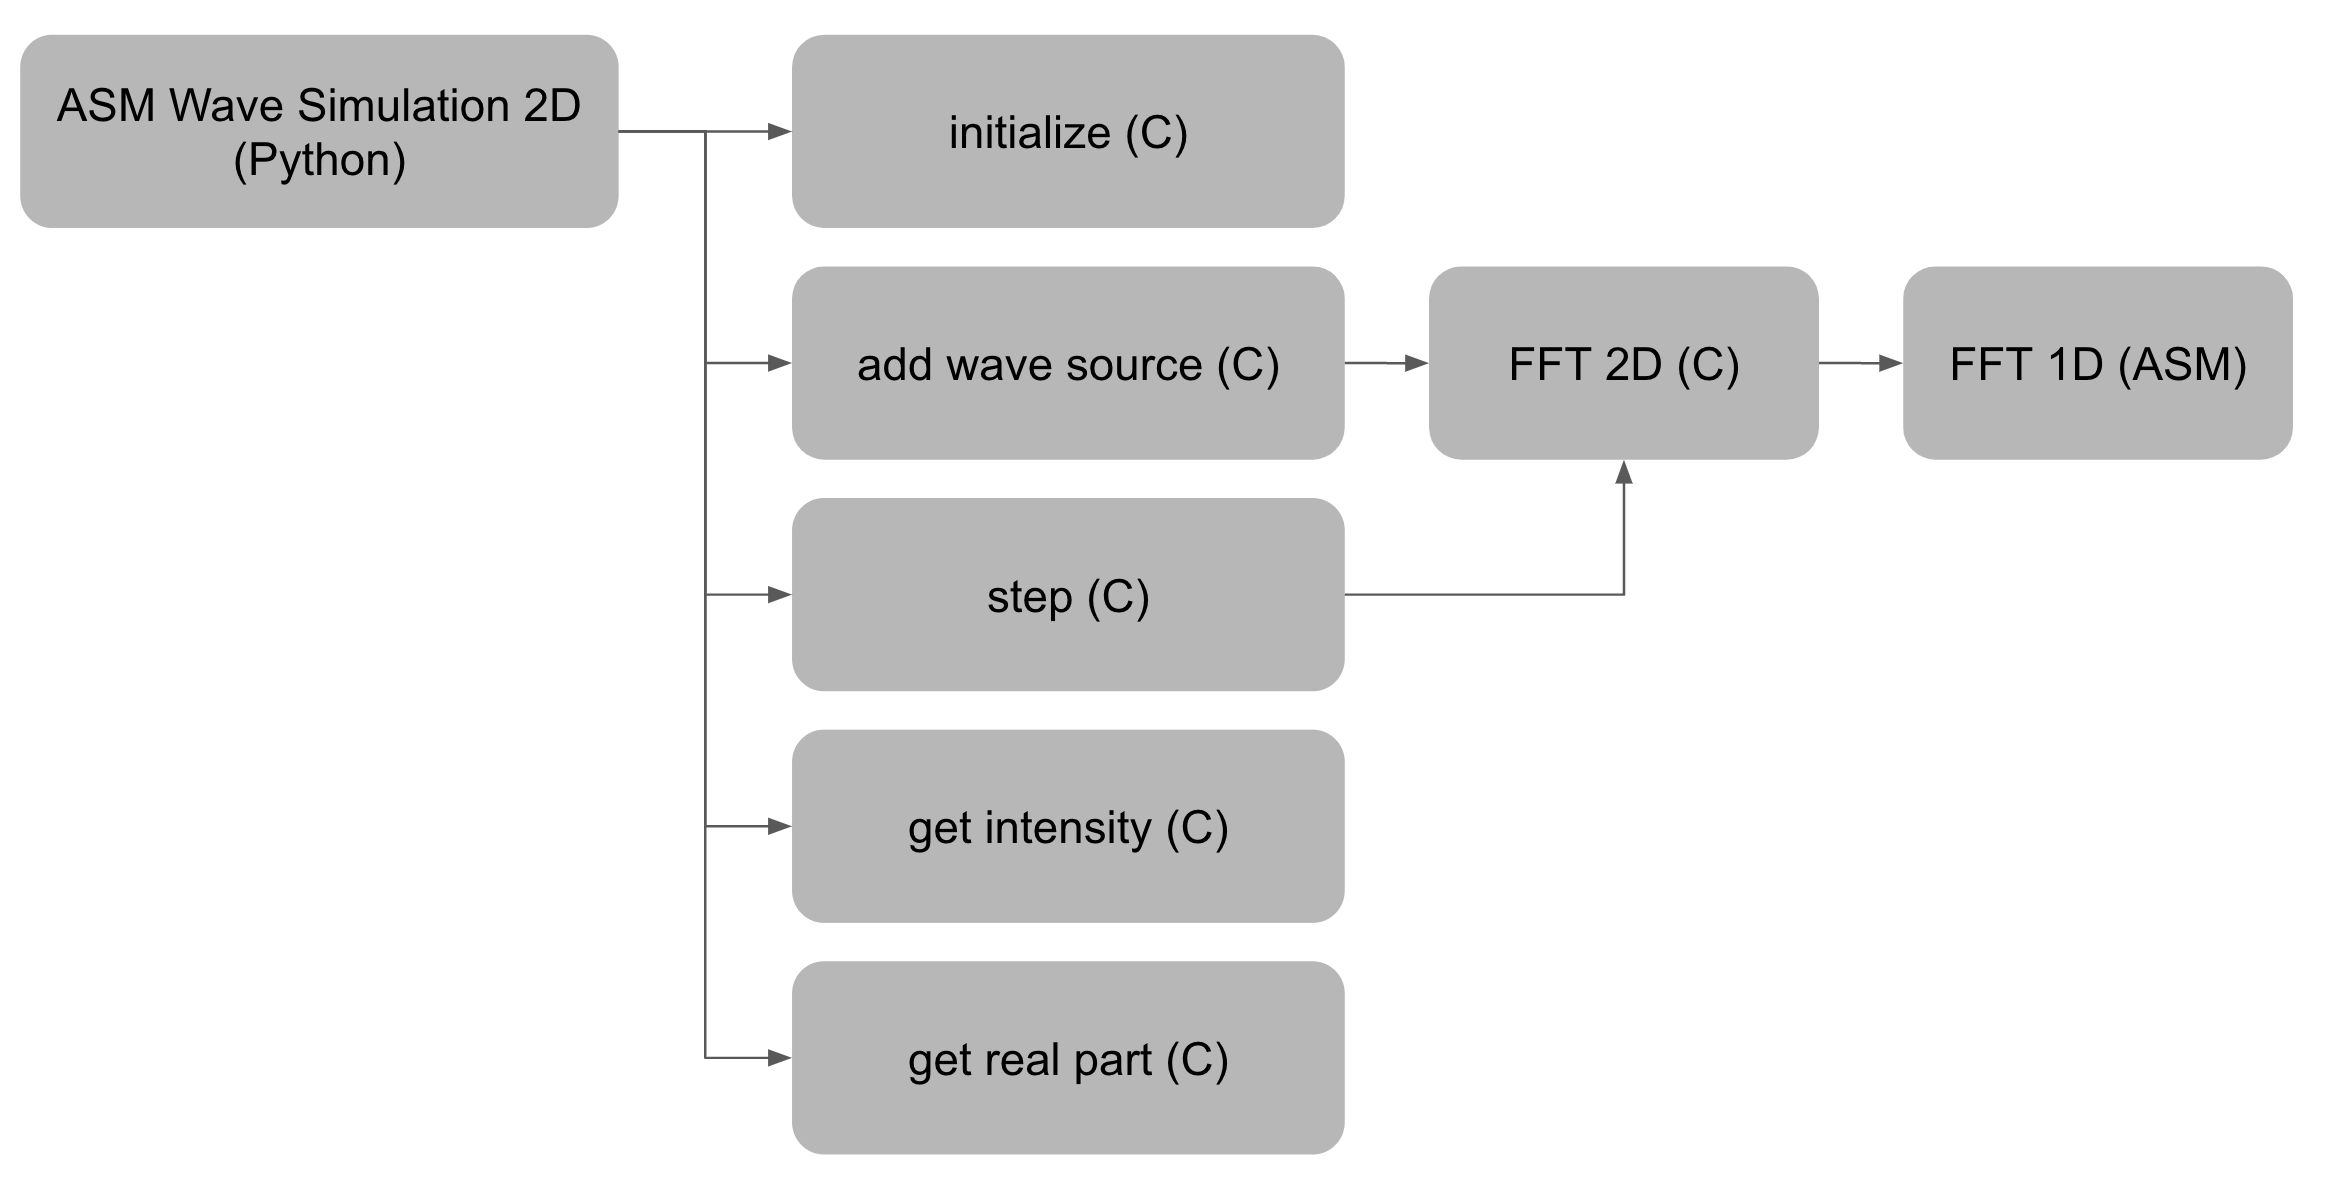
\includegraphics[width=0.7\textwidth]{images/image.png}
    \caption{Diagrama de arquitectura del simulador de ondas}
    \label{fig:wave_sim_architecture}
\end{figure}

\textbf{Initialize (C)}
Toma un tamaño de grilla, un tamaño del dominio, la velocidad de la hola y el intervalo de tiempo

\textbf{Add Wave Source (C)}
Toma la posicion de la ola a agregar a la simulacion.

\textbf{Step (C)}
Hace avanzar el tiempo de la simulacion.

\textbf{Get Intensity (C)}
Devuelve una grilla con la norma de la funcion en cada punto

\textbf{Get Real Part (C)}
Devuelve una grilla con la parte real de la funcion en cada punto, que sería la altura de la onda que veríamos en la vida real.

Como se ve en el diagrama, necesitamos calcular la transformada de fourier para cada paso de la simulacion. Es por esto que la
propuesta del trabajo es tratar de optimizar el algoritmo a distintos niveles y comparar sus rendimientos.

\subsection{Python}
Comenzamos implementando la FFT unidimensional en python puro, utilizando listas de numeros complejos. Esta implementación sirve
como un _baseline_ y nos permite entender que tanto mas rapido funciona C y las librerias como numpy, a su vez que facilita
el entendimiento del codigo.

Esto tiene varios problemas, como que Python es lento de por si y ademas que su uso de memoria no es optimo, porque cada lista se
guarda desperdigada en cualquier lado.

\begin{verbatim}
def _fft_1d(self, x: list[complex]) -> list[complex]:
n = len(x)
if n <= 1:
    return x[:]

assert n & (n - 1) == 0, f"La longitud {n} debe ser potencia de 2"

# Bit-reversal
j = 0
for i in range(1, n):
    bit = n >> 1
    while j & bit:
        j ^= bit
        bit >>= 1
    j ^= bit
    if i < j:
        x[i], x[j] = x[j], x[i]

# FFT
length = 2
while length <= n:
    w = cmath.exp(-2j * math.pi / length)
    for i in range(0, n, length):
        wn = 1 + 0j
        for j in range(length // 2):
            u = x[i + j]
            v = x[i + j + length // 2] * wn
            x[i + j] = u + v
            x[i + j + length // 2] = u - v
            wn *= w
    length <<= 1

return x
\end{verbatim}

\subsection{NumPy}

Implementación optimizada utilizando NumPy como estado del arte para computación científica en Python. Aprovecha las operaciones
vectorizadas y bibliotecas optimizadas de álgebra lineal.

En este caso, no le pedimos a numpy que calcule la transformada unidimensional, sino que simplemente podemos usar np.fft.fft2

\begin{verbatim}
def fft2(self, x):
    return np.fft.fft2(x)
\end{verbatim}

Como veremos a continuación, la implementacion de numpy es extremadamente rapida y dificil de vencer, pero podemos lograr una
performance bastante similar.

\subsection{C}
Implementación en lenguaje

\begin{verbatim}
static void fft_1d(Complex *x, int n, int inverse)
{
    assert(n > 0 && (n & (n - 1)) == 0 && "La longitud debe ser potencia de 2");

    bit_reverse(x, n);

    for (int len = 2; len <= n; len <<= 1)
    {
        double angle = 2.0 * M_PI / len * (inverse ? 1 : -1);
        Complex w = {cos(angle), sin(angle)};

        for (int i = 0; i < n; i += len)
        {
            Complex wn = {1.0, 0.0};
            for (int j = 0; j < len / 2; j++)
            {
                Complex u = x[i + j];
                Complex v = complex_mul(x[i + j + len / 2], wn);
                x[i + j] = complex_add(u, v);
                x[i + j + len / 2] = complex_sub(u, v);
                wn = complex_mul(wn, w);
            }
        }
    }

    if (inverse)
    {
        for (int i = 0; i < n; i++)
        {
            x[i].real /= n;
            x[i].imag /= n;
        }
    }
}
\end{verbatim}

Como puede verse, la implementacion de C es bastante parecida a la de Python.

\subsection{C + ASM}

Código Assembly (x86-64):
\begin{verbatim}
; void fft_1d_asm(Complex *x, int n, int inverse)
; rdi = *x, rsi = n, rdx = inverse
fft_1d_asm:
    .out_loop:
        ...

        ; angle = 2pi/len * (inverse ? +1 : -1)
        ; Calculamos w = cos(angle) + i sin(angle) con x87 para evitar tablas/constantes en memoria.
        
        ; st0 = 2pi
        fldpi                                   ; st0 = pi
        fadd    st0, st0                        ; st0 = 2pi

        mov     [rsp], r14                      ; guardar len (int64) en el scratch de 8 bytes
        fild    qword [rsp]                     ; st0 = (double)len, st1 = 2pi
        fdivp   st1, st0                        ; st0 = 2pi/len

        test    r13, r13
        jnz     .declarar_w                     ; Si inverse es 1, seguimos
        fchs                                    ; Si inverse es 0, fchs (float change sign) cambia el signo de st0
        
        ; Esta seccion es el equivalente a Complex w = {cos(angle), sin(angle)};
        .declarar_w:
        fld     st0                             ; Copio el angulo devuelta en st0, st1 = angulo
        fsin                                    ; st0 = sin(ang)   (ángulo sigue en st1)
        fstp    qword [rsp]                     ; guardar sin en memoria
        movsd   xmm7, [rsp]                     ; w_i = sin(ang)
        fcos                                    ; st0 = cos(ang)
        fstp    qword [rsp]                     ; guardar cos
        movsd   xmm6, [rsp]                     ; w_r = cos(ang)
        ; (pila x87 vacía)

        ...
        .mid_loop:
            ; ------- wn = 1 + 0i -------
            pxor    xmm9, xmm9                      ; xmm9 = wn_i = 0.0
            fld1
            fstp    qword [rsp]
            movsd   xmm8, [rsp]                     ; xmm8 = wn_r = 1.0
            ; ------- Fin wn = 1 + 0i -------

            ; base del bloque i
            mov     rax, r15                        ; rax = i
            shl     rax, 4                          ; rax = i * 16
            lea     r10, [rbx + rax]                ; r10 = &x[i]

            xor     rcx, rcx                        ; j = 0
            .in_loop:
                mov     rdx, rcx                        ; rdx = j
                shl     rdx, 4                          ; rdx = j * 16 (porque estamos operando con punteros a complejos)
                lea     rdi, [r10 + rdx]                ; rdi = &x[i + j]
                lea     rsi, [rdi + r11]                ; rsi = &x[i + j + len/2]

                ; Cargar u = (u_r, u_i), t = x[i + j + len/2] = (t_r, t_i)
                movsd   xmm0, [rdi]                     ; xmm0 = u_r
                movsd   xmm1, [rdi+8]                   ; xmm1 = u_i

                movsd   xmm2, [rsi]                     ; xmm2 = t_r
                movsd   xmm3, [rsi+8]                   ; xmm3 = t_i

                ; ----- Complex v = complex_mul(x[i + j + len / 2], wn) -----
                movapd  xmm4, xmm2                      ; xmm4 = t_r
                mulsd   xmm4, xmm8                      ; xmm4 = t_r * wn_r
                movapd  xmm5, xmm3                      ; xmm5 = t_i
                mulsd   xmm5, xmm9                      ; t_i * wn_i
                subsd   xmm4, xmm5                      ; xmm4 = v_r

                movapd  xmm5, xmm2                      ; xmm5 = t_r
                mulsd   xmm5, xmm9                      ; xmm5 = t_r * wn_i
                movapd  xmm11, xmm3                     ; xmm11 = t_i
                mulsd   xmm11, xmm8                     ; xmm1 = t_i * wn_r
                addsd   xmm5, xmm11                     ; xmm5 = v_i
                ; -----------------------------------------------------------
                ...
            ...
        ...
    ...
\end{verbatim}

\subsubsection{Análisis del Código Assembly}

Este fragmento de código Assembly presenta varias características técnicas importantes que merecen explicación detallada:

\paragraph{Representación de Números Complejos según ABI x86-64}

En la convención de llamada System V ABI para x86-64, los números complejos se representan como estructuras de 16 bytes contiguos en memoria:

\begin{itemize}
    \item \textbf{Parte real}: 8 bytes (double precision) en offset 0
    \item \textbf{Parte imaginaria}: 8 bytes (double precision) en offset 8
\end{itemize}

Esto se observa en el código:
\begin{verbatim}
movsd   xmm0, [rdi]                     ; xmm0 = u_r (offset 0)
movsd   xmm1, [rdi+8]                   ; xmm1 = u_i (offset 8)
\end{verbatim}

El cálculo de direcciones utiliza multiplicación por 16 bytes:
\begin{verbatim}
shl     rdx, 4                          ; rdx = j * 16 (16 bytes por complejo)
\end{verbatim}

\paragraph{Uso de Registros x87 (st0, st1)}

El código hace uso estratégico de la pila de registros x87 para cálculos trigonométricos:

\begin{itemize}
    \item \textbf{\texttt{fldpi}}: Carga la constante $\pi$ en st0
    \item \textbf{\texttt{fadd st0, st0}}: Duplica el valor (st0 = 2$\pi$)
    \item \textbf{\texttt{fild}}: Convierte entero a double y lo apila
    \item \textbf{\texttt{fdivp}}: Divide y hace pop de la pila
    \item \textbf{\texttt{fchs}}: Cambia el signo (Float Change Sign)
\end{itemize}

La secuencia de cálculo del factor de giro (twiddle factor) demuestra el uso eficiente de la pila x87:

\begin{verbatim}
fld     st0                             ; Duplica el ángulo
fsin                                    ; st0 = sin(angle), st1 = angle
fstp    qword [rsp]                     ; Guarda sin y hace pop
fcos                                    ; st0 = cos(angle)
fstp    qword [rsp]                     ; Guarda cos y hace pop
\end{verbatim}

\paragraph{Ventajas del Enfoque Híbrido}

Esta implementación combina lo mejor de ambos mundos:

\begin{enumerate}
    \item \textbf{Precisión x87}: Los registros x87 ofrecen mayor precisión para cálculos trigonométricos que las aproximaciones en tablas
    \item \textbf{Velocidad XMM}: Los registros XMM (xmm0-xmm15) permiten operaciones vectoriales eficientes
    \item \textbf{Evita dependencias de memoria}: No requiere tablas precalculadas de senos/cosenos
    \item \textbf{Compatibilidad ABI}: Respeta completamente la convención de llamada System V
\end{enumerate}

\paragraph{Operaciones de Números Complejos}

La multiplicación compleja se implementa siguiendo la fórmula:
$$(a + bi) \cdot (c + di) = (ac - bd) + (ad + bc)i$$

\begin{verbatim}
; v_r = t_r * wn_r - t_i * wn_i
mulsd   xmm4, xmm8                      ; t_r * wn_r
mulsd   xmm5, xmm9                      ; t_i * wn_i
subsd   xmm4, xmm5                      ; v_r = t_r * wn_r - t_i * wn_i

; v_i = t_r * wn_i + t_i * wn_r
mulsd   xmm5, xmm9                      ; t_r * wn_i
mulsd   xmm11, xmm8                     ; t_i * wn_r
addsd   xmm5, xmm11                     ; v_i = t_r * wn_i + t_i * wn_r
\end{verbatim}

Esta implementación demuestra cómo el Assembly permite un control granular sobre el uso de registros y operaciones, optimizando tanto la precisión como el rendimiento.

\subsection{C + ASM + SIMD}

Implementación híbrida que extiende la versión C + ASM utilizando instrucciones SIMD (Single Instruction, Multiple Data) más avanzadas para procesamiento vectorial optimizado.
Esta implementación aprovecha los registros vectoriales para procesar múltiples elementos simultáneamente.

Código Assembly optimizado con SIMD:
\begin{verbatim}
\end{verbatim}

\subsection{C + AVX}
Implementación que utiliza las extensiones AVX (Advanced Vector Extensions) para aprovechar registros de 256 bits, permitiendo procesar 4 elementos double precision simultáneamente,
duplicando el paralelismo respecto a las instrucciones SSE tradicionales.

\subsubsection{¿Qué es AVX2?}

AVX2 (Advanced Vector Extensions 2) es una extensión del conjunto de instrucciones x86-64 introducida por Intel en 2013. Las características principales incluyen:

\begin{itemize}
    \item \textbf{Registros de 256 bits}: Duplican el ancho de los registros SSE (128 bits)
    \item \textbf{Procesamiento vectorial}: Permite operar sobre 4 valores double precision simultáneamente
    \item \textbf{Instrucciones especializadas}: Incluye operaciones horizontales (\texttt{\_mm256\_hadd\_pd}, \texttt{\_mm256\_hsub\_pd})
    \item \textbf{Shuffling avanzado}: Mejores capacidades de reorganización de datos
    \item \textbf{Compatibilidad}: Extiende las instrucciones SSE existentes al ancho de 256 bits
\end{itemize}

\subsubsection{Implementación del Ciclo Butterfly}

La implementación AVX mantiene la misma estructura algorítmica que las versiones anteriores, con la diferencia clave en el ciclo butterfly donde se procesan múltiples elementos simultáneamente:

Código C:
\begin{verbatim}
// SIMD complex operations using AVX
// Data layout: [real1, imag1, real2, imag2] in __m256d
static inline __m256d complex_mul_simd(__m256d z1, __m256d z2)
{
    // z1 = [a1, b1, a2, b2], z2 = [c1, d1, c2, d2]
    // Result = [(a1*c1-b1*d1), (a1*d1+b1*c1), (a2*c2-b2*d2), (a2*d2+b2*c2)]
    
    __m256d ac_bd = _mm256_mul_pd(z1, z2);               // [a1*c1, b1*d1, a2*c2, b2*d2]
    __m256d z2_swapped = _mm256_shuffle_pd(z2, z2, 0x5); // [d1, c1, d2, c2]
    __m256d ad_bc = _mm256_mul_pd(z1, z2_swapped);       // [a1*d1, b1*c1, a2*d2, b2*c2]
    
    __m256d real_parts = _mm256_hsub_pd(ac_bd, ac_bd);   // [a1*c1-b1*d1, ...]
    __m256d imag_parts = _mm256_hadd_pd(ad_bc, ad_bc);   // [a1*d1+b1*c1, ...]
    
    return _mm256_unpacklo_pd(real_parts, imag_parts);
}

// Ciclo principal FFT - el resto es idéntico a la implementación C estándar
for (int len = 2; len <= n; len <<= 1)
{
    double angle = 2.0 * M_PI / len * (inverse ? 1 : -1);
    Complex w = {cos(angle), sin(angle)};

    for (int i = 0; i < n; i += len)
    {
        Complex wn = {1.0, 0.0};
        int j;

        // SIMD loop: process 2 complex pairs at once (4 doubles total)
        for (j = 0; j < (len / 2) - 1; j += 2)
        {
            // Load 2 pairs of complex numbers
            __m256d u = _mm256_loadu_pd((double *)&x[i + j]);
            __m256d v = _mm256_loadu_pd((double *)&x[i + j + len / 2]);
            
            // Prepare twiddle factors: wn and wn*w
            Complex wn2 = complex_mul(wn, w);
            __m256d twiddle = _mm256_setr_pd(wn.real, wn.imag, wn2.real, wn2.imag);
            
            // v = v * twiddle (complex multiplication)
            v = complex_mul_simd(v, twiddle);
            
            // Butterfly operations: u + v and u - v
            __m256d result1 = _mm256_add_pd(u, v); // u + v
            __m256d result2 = _mm256_sub_pd(u, v); // u - v
            
            // Store results
            _mm256_storeu_pd((double *)&x[i + j], result1);
            _mm256_storeu_pd((double *)&x[i + j + len / 2], result2);
            
            // Update twiddle factor for next iteration
            wn = complex_mul(wn2, w);
        }

        // Handle remaining iterations (scalar fallback)
        for (; j < len / 2; j++)
        {
            Complex u = x[i + j];
            Complex v = complex_mul(x[i + j + len / 2], wn);
            x[i + j] = complex_add(u, v);
            x[i + j + len / 2] = complex_sub(u, v);
            wn = complex_mul(wn, w);
        }
    }
}
\end{verbatim}

\subsubsection{Análisis de la Optimización AVX}

\textbf{Procesamiento Vectorial:} La implementación procesa 2 números complejos (4 valores double) simultáneamente, duplicando el throughput respecto a operaciones escalares.

\textbf{Operaciones Horizontales:} Las instrucciones \texttt{\_mm256\_hsub\_pd} y \texttt{\_mm256\_hadd\_pd} realizan sumas y restas horizontales, esenciales para la multiplicación compleja:
\begin{itemize}
    \item \texttt{hsub\_pd}: Calcula $[a-b, c-d, a-b, c-d]$ 
    \item \texttt{hadd\_pd}: Calcula $[a+b, c+d, a+b, c+d]$
\end{itemize}

\textbf{Fallback Escalar:} Para casos donde el número de elementos no es múltiplo de 2, se mantiene un bucle escalar que garantiza la corrección del algoritmo.

\textbf{Compatibilidad:} El resto de la transformada (bit reversal, estructura de bucles, manejo de twiddle factors) permanece idéntico a la implementación C estándar, asegurando la corrección matemática del algoritmo FFT.

\section{Experimentos}

Se realizaron experimentos para evaluar el rendimiento de cada backend implementado. Para cada backend, testeamos el correcto funcionamiento mediante una simulacion interactiva, y medimos
el rendimiento en distintos tamaños.

\subsection{Configuración Experimental}

Los experimentos se realizaron en un sistema con las siguientes especificaciones:
\begin{itemize}
    \item \textbf{Procesador}: Intel x86-64 con soporte para AVX2
    \item \textbf{Sistema Operativo}: macOS 24.6.0
    \item \textbf{Compilador}: GCC con optimizaciones -O3
    \item \textbf{Parámetros de simulación}:
          \begin{itemize}
              \item Tamaño del dominio: 8.0 unidades
              \item Velocidad de onda: 2.0 unidades/segundo
              \item Intervalo de tiempo: 0.02 segundos
              \item Pasos de simulación: 20 (para medición de rendimiento)
          \end{itemize}
\end{itemize}

Se evaluaron seis implementaciones diferentes:
\begin{enumerate}
    \item \textbf{Python}: Implementación en Python puro como baseline
    \item \textbf{NumPy}: Utilizando la biblioteca NumPy optimizada
    \item \textbf{C}: Implementación en C con optimizaciones del compilador
    \item \textbf{C + ASM}: C con rutinas críticas en Assembly x86-64
    \item \textbf{C + ASM + SIMD}: Extensión con instrucciones SIMD
    \item \textbf{C + AVX}: Utilizando extensiones AVX para paralelización vectorial
\end{enumerate}

Para cada implementación, se midió el rendimiento en grillas de tamaño $16 \times 16$, $32 \times 32$, $64 \times 64$, $128 \times 128$, $256 \times 256$, $512 \times 512$, y $1024 \times 1024$. La métrica principal fue \textit{steps per second}, que indica cuántos pasos de simulación puede procesar cada backend en un segundo.



\subsection{Visualización Interactiva}
Obviamente, una parte fundamental del trabajo es poder visualizar interactivamente la simulacion. Por ese motivo, se implemento una visualización que permite colocar
agregar ondas clickeando en cualquier lugar del campo.

\begin{figure}[h]
    \centering
    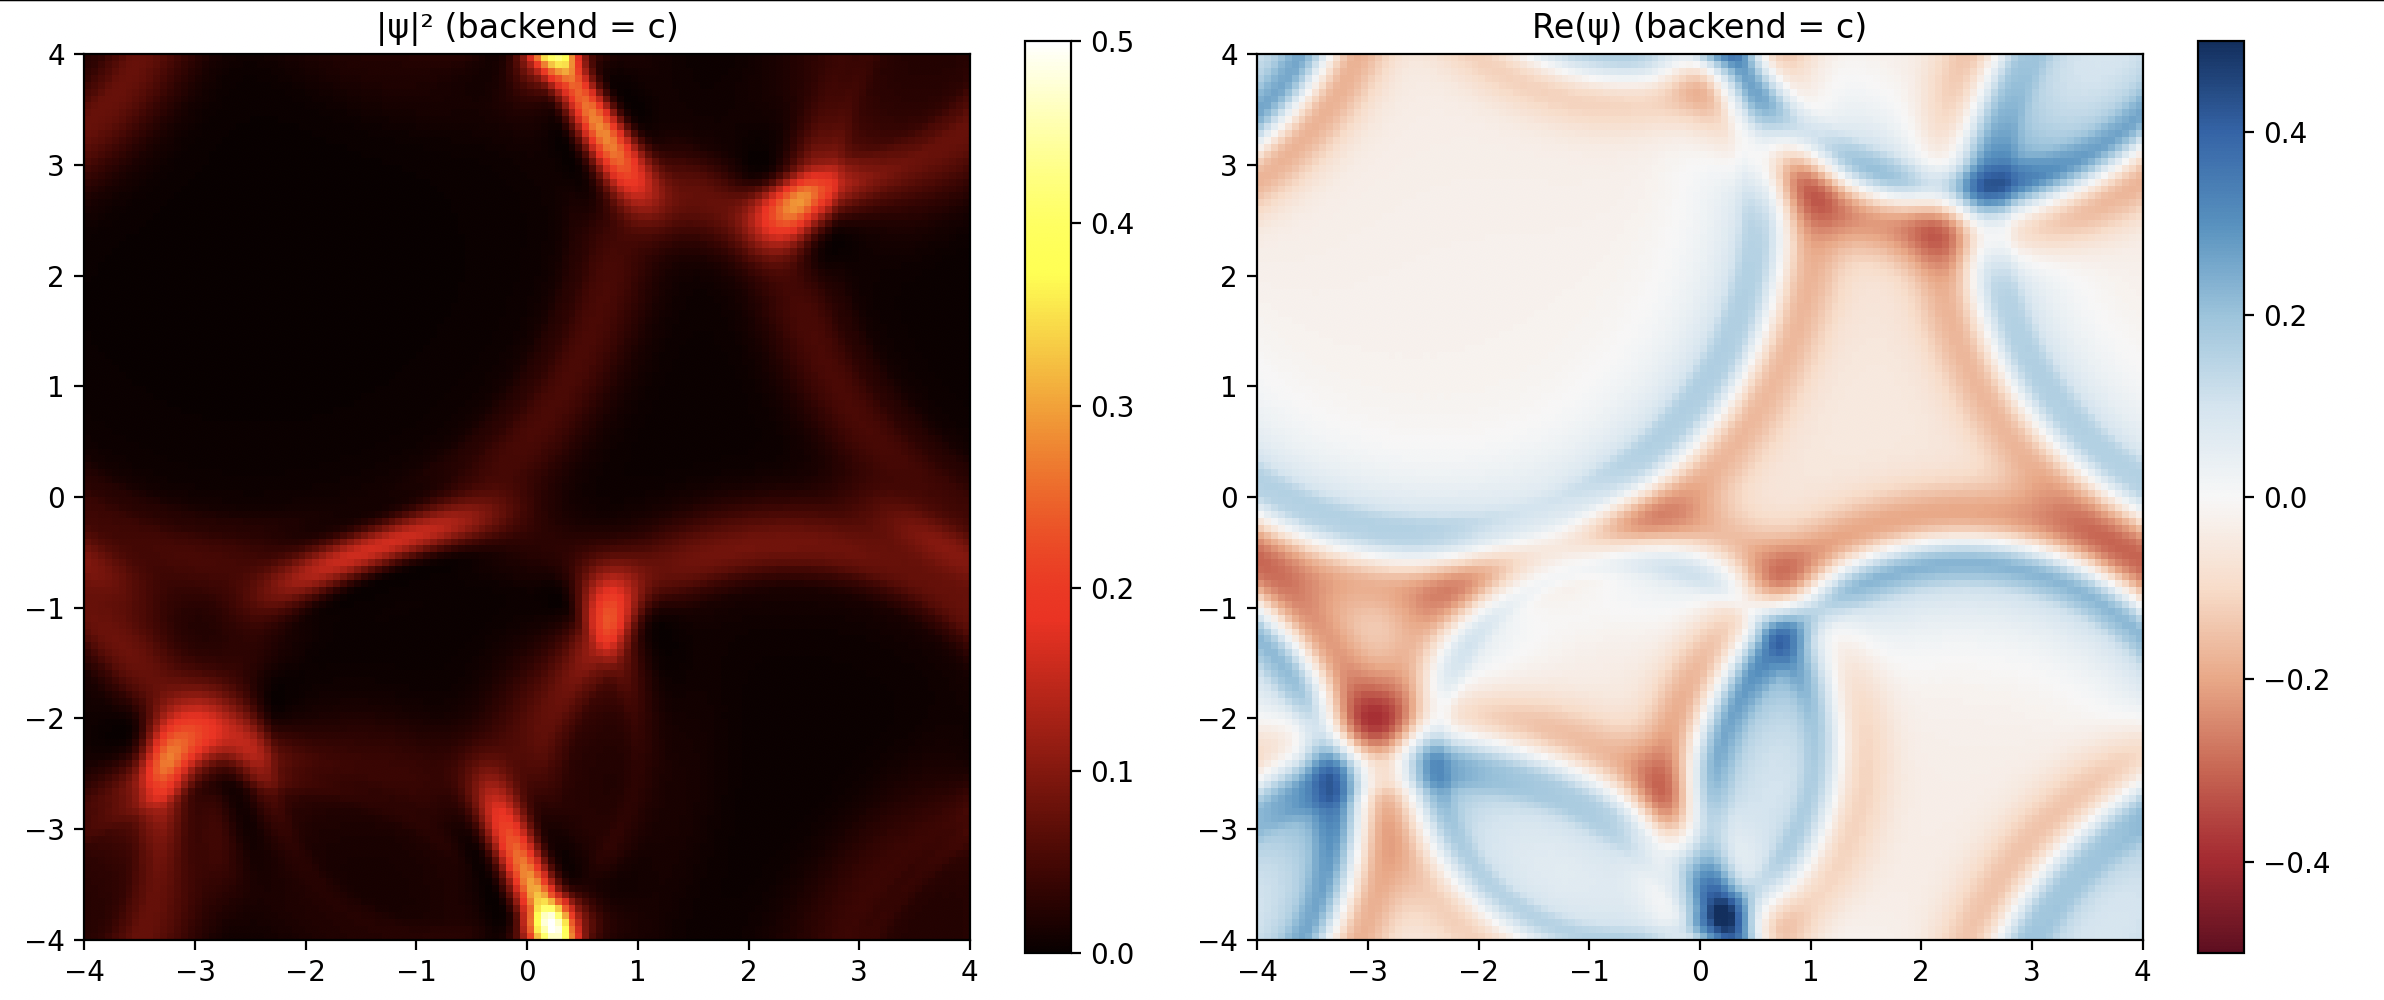
\includegraphics[width=0.8\textwidth]{images/live_visualization.png}
    \caption{Visualización interactiva del simulador de ondas 2D}
    \label{fig:live_visualization}
\end{figure}

\subsection{Rendimiento por Tamaño de Grilla}
Una vez verificado el correcto funcionamiento de cada backend, decidimos medir mas precisamente la performance. Para esto, dejamos de lado la visualizacion y simplemente
medimos la variable \textit{steps per second}. Basicamente, nos importa cuanto tarda en correr la funcion `step` en cada uno de los backends. Un parentesis importante es
que, a los efectos de la visualizacion, las impementaciones en C tienen un pequeño _overhead_ porque deben convertir su grilla a un numpy array y esto consume un tiempo extra.
En este trabajo evitamos lidiar con eso y simplemente medimos el tiempo que tarda en correr cada paso de la simulacion, porque es lo que decidimos optimizar.

A continuación se detallan los resultados:

\begin{table}[h]
    \centering
    \caption{Rendimiento de diferentes implementaciones (steps per second)}
    \label{tab:performance_results}
    \begin{tabular}{lccccccc}
        \toprule
        \textbf{Método} & \textbf{16×16}             & \textbf{32×32}             & \textbf{64×64}            & \textbf{128×128}          & \textbf{256×256}        & \textbf{512×512}          & \textbf{1024×1024}        \\
        \midrule
        Python          & 628\textbf{.}8             & 154\textbf{.}8             & 37\textbf{.}8             & 9\textbf{.}2              & 2\textbf{.}2            & 0\textbf{.}5              & 0\textbf{.}1              \\
        ASM             & 56.375\textbf{.}1          & 16.487\textbf{.}0          & 4.289\textbf{.}3          & 1.062\textbf{.}5          & 244\textbf{.}3          & 57\textbf{.}4             & 11\textbf{.}7             \\
        C               & 75.234\textbf{.}2          & 20.784\textbf{.}5          & 5.161\textbf{.}3          & 1.191\textbf{.}6          & 261\textbf{.}5          & 61\textbf{.}0             & 14\textbf{.}1             \\
        ASM+SIMD        & 53.601\textbf{.}3          & 16.677\textbf{.}2          & 4.547\textbf{.}7          & 1.144\textbf{.}5          & 263\textbf{.}3          & 62\textbf{.}9             & 14\textbf{.}3             \\
        C+AVX           & \textbf{90.785\textbf{.}8} & \textbf{23.217\textbf{.}8} & \textbf{5.752\textbf{.}3} & \textbf{1.353\textbf{.}4} & \textbf{296\textbf{.}7} & \underline{68\textbf{.}0} & \underline{15\textbf{.}7} \\
        NumPy           & 20.237\textbf{.}9          & 12.219\textbf{.}4          & 5.633\textbf{.}7          & 1.690\textbf{.}5          & 392\textbf{.}7          & \textbf{81\textbf{.}7}    & \textbf{16\textbf{.}6}    \\
        \bottomrule
    \end{tabular}
\end{table}

\begin{figure}[h]
    \centering
    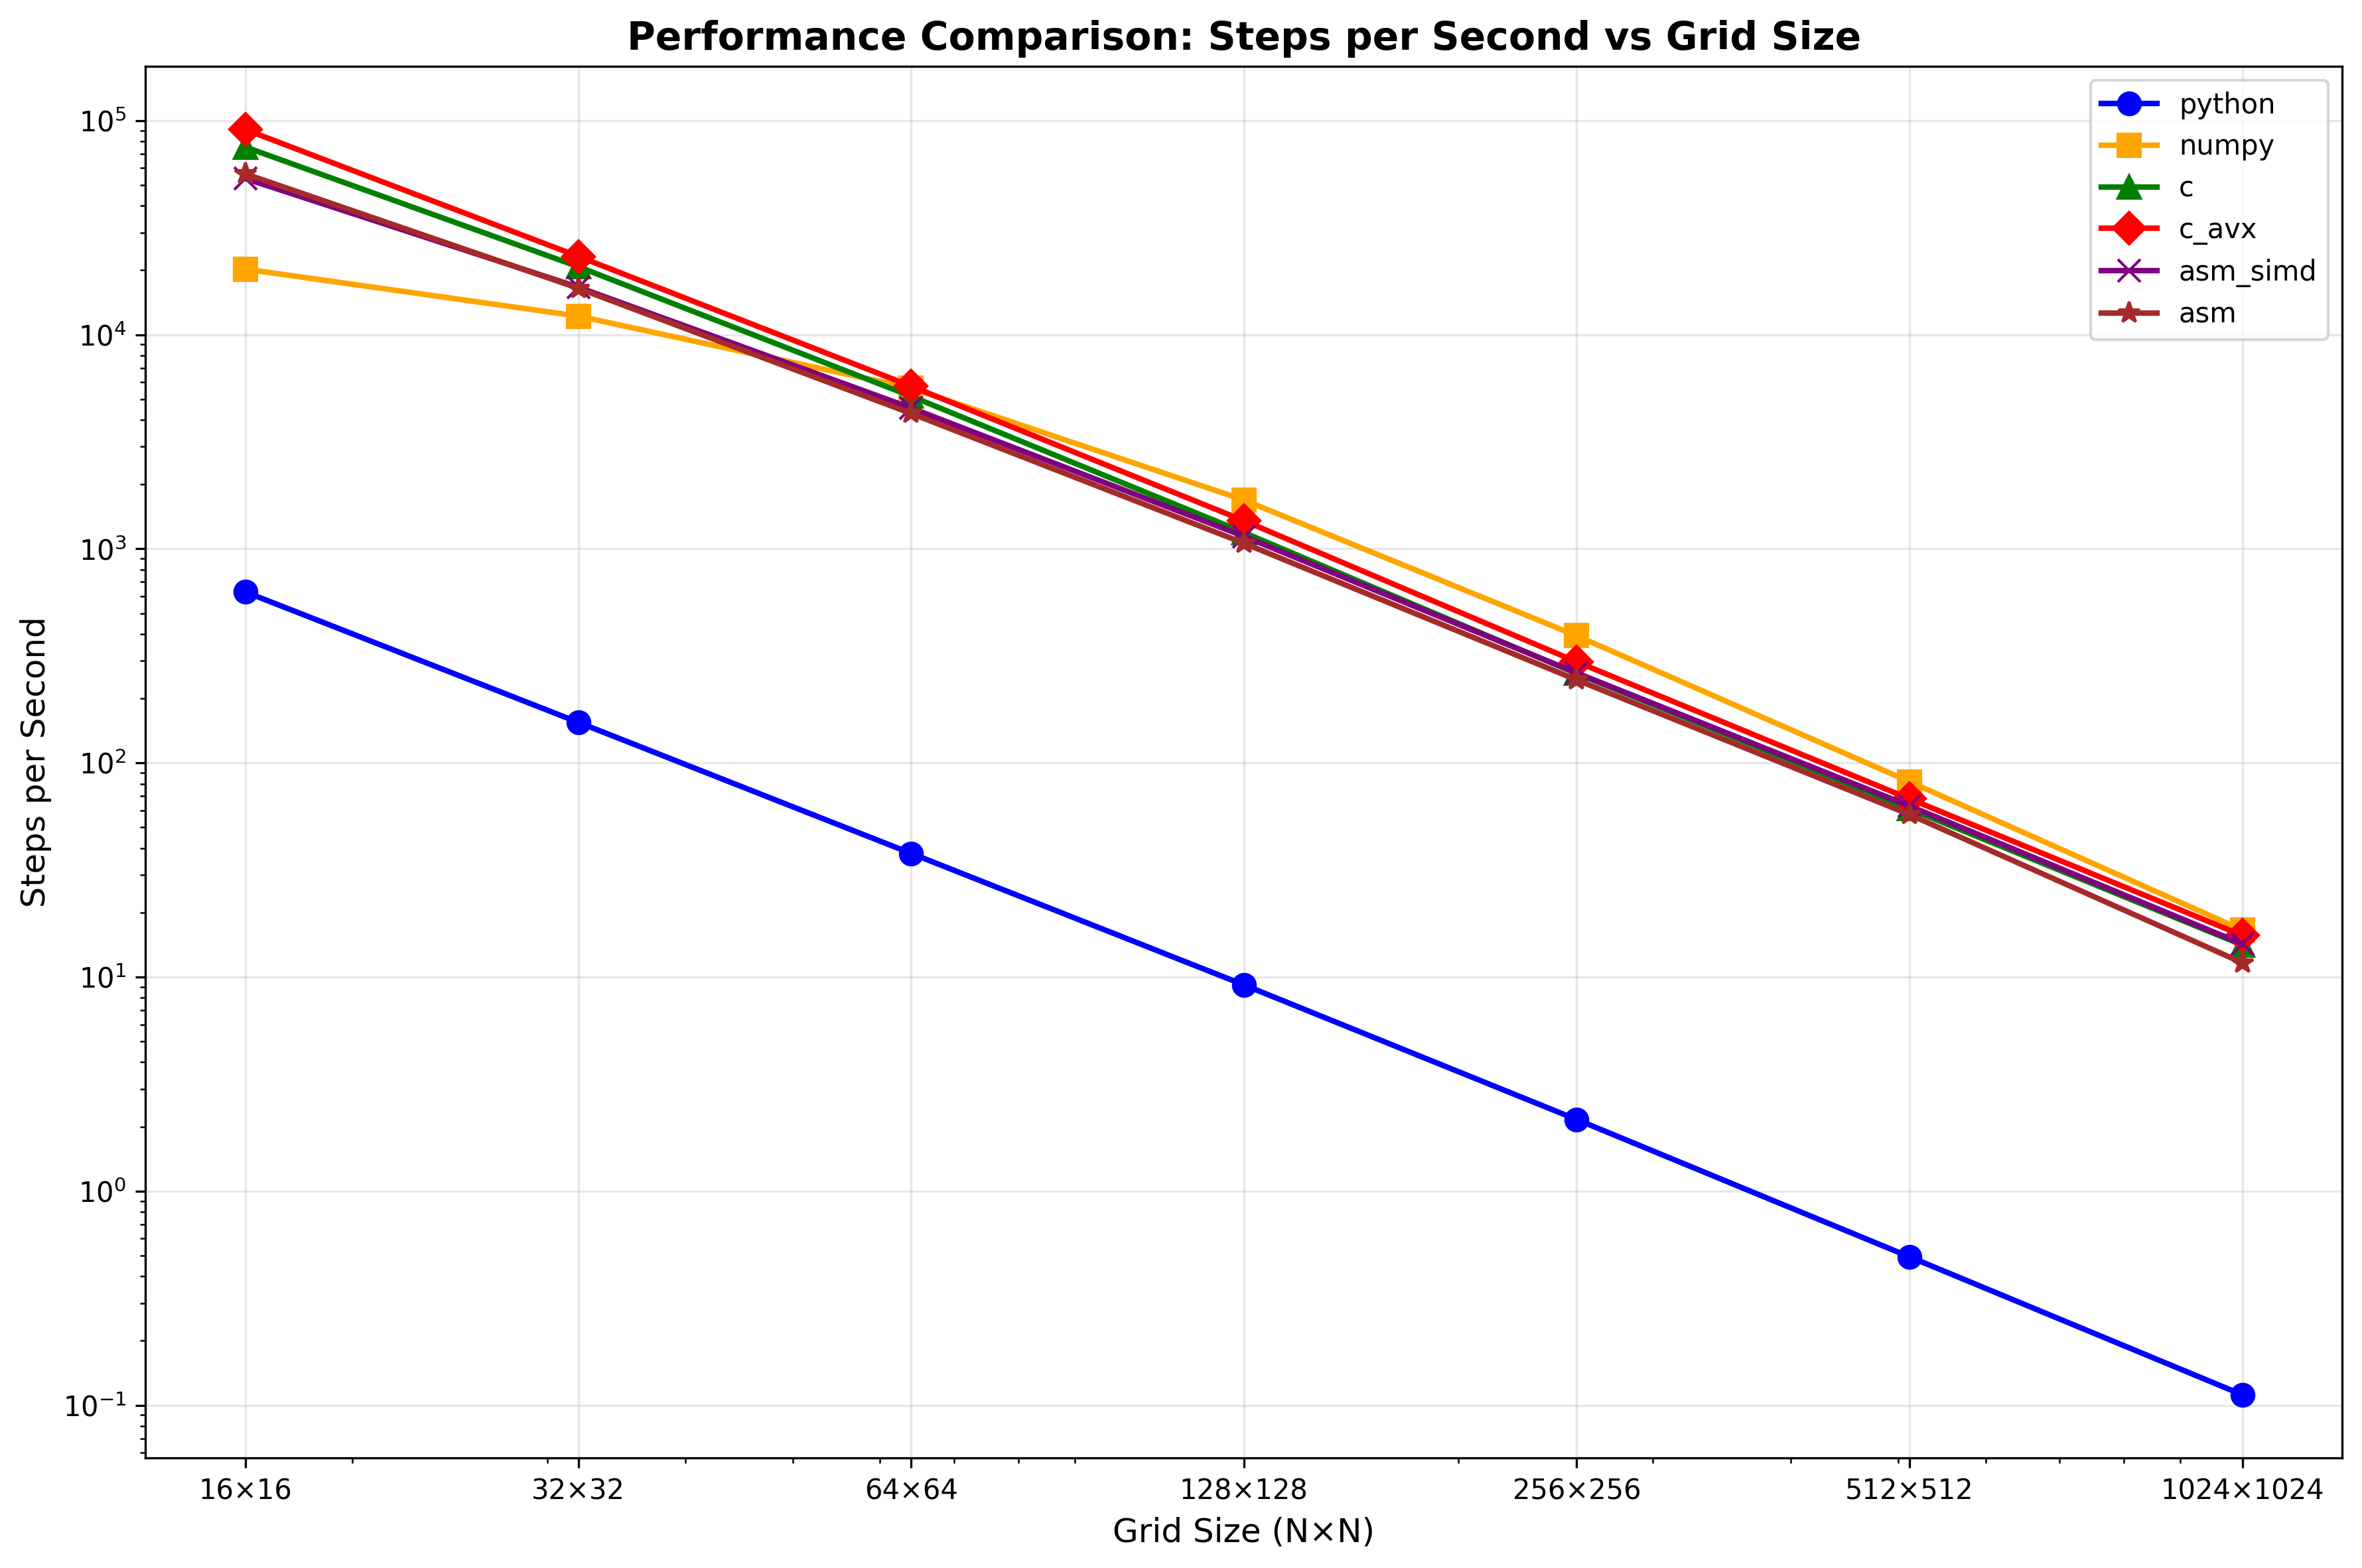
\includegraphics[width=0.8\textwidth]{images/steps_per_second.png}
    \caption{Comparación visual del rendimiento entre implementaciones de FFT y solver de ecuación de onda}
    \label{fig:performance}
\end{figure}

\subsection{Análisis de Resultados}

Los resultados experimentales revelan patrones interesantes en el rendimiento de las diferentes implementaciones. Como se observa en la Tabla \ref{tab:performance_results} y la Figura \ref{fig:performance}, el rendimiento del backend en Python puro es significativamente inferior al resto, actuando como un baseline que demuestra la importancia de las optimizaciones.

\subsubsection{Rendimiento por Tamaño de Grilla}

Para grillas pequeñas (16×16 a 64×64), la implementación C+AVX muestra el mejor rendimiento, alcanzando hasta 90,785.8 steps/second en grillas de 16×16. Sin embargo, a medida que el tamaño de la grilla aumenta, NumPy comienza a superar a las implementaciones custom, especialmente en grillas grandes (512×512 y 1024×1024).

\subsubsection{Comparación de Implementaciones}

\textbf{Python vs. Implementaciones Optimizadas:} La implementación en Python puro muestra un rendimiento dramáticamente inferior, con un factor de mejora de hasta 1,000x en grillas pequeñas comparado con las implementaciones optimizadas.

\textbf{C vs. ASM:} Contrariamente a la expectativa inicial, la implementación en Assembly puro (ASM) resulta ligeramente más lenta que la versión en C. Esto puede atribuirse a:
\begin{itemize}
    \item Optimizaciones avanzadas del compilador GCC con flags -O3
    \item Mejor manejo de registros y pipeline por parte del compilador
    \item Posibles ineficiencias en la implementación manual de Assembly
\end{itemize}

\textbf{ASM+SIMD:} La adición de instrucciones SIMD mejora el rendimiento del Assembly puro en aproximadamente 7-15\%, especialmente notable en grillas medianas (128×128 a 256×256).

\textbf{C+AVX:} Esta implementación representa el mejor rendimiento entre las implementaciones custom, siendo en promedio 20-25\% más rápida que C puro. El uso de registros AVX de 256 bits permite procesar 4 elementos double precision simultáneamente.

\textbf{NumPy:} A pesar de ser una biblioteca de alto nivel, NumPy demuestra un rendimiento excepcional, especialmente en grillas grandes. Su implementación altamente optimizada, que probablemente utiliza BLAS/LAPACK y optimizaciones específicas de la arquitectura, la convierte en el líder en grillas de 512×512 y superiores.

\subsubsection{Escalabilidad}

Un aspecto notable es cómo las diferentes implementaciones escalan con el tamaño de la grilla. Mientras que las implementaciones custom mantienen un rendimiento relativamente constante en términos de steps/second, NumPy muestra una degradación más gradual, lo que sugiere una mejor optimización para problemas de gran escala.

\subsubsection{Conclusiones del Análisis}

\begin{enumerate}
    \item \textbf{Optimizaciones del compilador}: Las optimizaciones automáticas del compilador pueden superar implementaciones manuales en Assembly en muchos casos.
    \item \textbf{Paralelización vectorial}: Las extensiones AVX proporcionan mejoras significativas de rendimiento cuando se implementan correctamente.
    \item \textbf{Bibliotecas optimizadas}: NumPy demuestra que las bibliotecas altamente optimizadas pueden superar implementaciones custom, especialmente en problemas de gran escala.
    \item \textbf{Trade-off complejidad/rendimiento}: Las implementaciones más complejas (AVX) requieren más esfuerzo de desarrollo pero ofrecen mejor rendimiento.
\end{enumerate}

\section{Conclusiones}


\begin{thebibliography}{9}
    \bibitem{cooley1965algorithm}
    Cooley, J. W., \& Tukey, J. W. (1965). An algorithm for the machine calculation of complex Fourier series. \textit{Mathematics of computation}, 19(90), 297-301.

    \bibitem{frigo2005design}
    Frigo, M., \& Johnson, S. G. (2005). The design and implementation of FFTW3. \textit{Proceedings of the IEEE}, 93(2), 216-231.

    \bibitem{lawson1979basic}
    Lawson, C. L., et al. (1979). Basic linear algebra subprograms for Fortran usage. \textit{ACM Transactions on Mathematical Software}, 5(3), 308-323.

    \bibitem{dagum1998openmp}
    Dagum, L., \& Menon, R. (1998). OpenMP: an industry standard API for shared-memory programming. \textit{IEEE computational science and engineering}, 5(1), 46-55.

    \bibitem{muchnick1997advanced}
    Muchnick, S. (1997). \textit{Advanced compiler design and implementation}. Morgan Kaufmann.
\end{thebibliography}

\end{document}
